% Study 6 evaluation report: Farm to Table (DCST.0824-0825)
% Compile: latexmk -pdf Study6_Evaluation_Report.tex   (figures: python make_figures.py)
\documentclass[11pt,a4paper]{article}

\usepackage[a4paper,margin=1in]{geometry}
\usepackage[T1]{fontenc}
\usepackage{newtxtext,newtxmath}
\usepackage[utf8]{inputenc}
\usepackage{microtype}
\usepackage{graphicx}
\usepackage{booktabs}
\usepackage{tabularx}
\usepackage{threeparttable}
\usepackage{makecell}
\usepackage{array}
\usepackage{float}
\usepackage{caption}
\usepackage{enumitem}
\usepackage{titlesec}
\usepackage[round]{natbib}
\usepackage[hidelinks]{hyperref}

\captionsetup{font=small,labelfont=bf,labelsep=period,justification=raggedright,singlelinecheck=false}
\captionsetup[table]{position=top,skip=4pt}
\captionsetup[figure]{skip=6pt}
\titleformat{\section}{\normalfont\large\bfseries}{\thesection}{0.6em}{}
\titleformat{\subsection}{\normalfont\normalsize\bfseries}{\thesubsection}{0.6em}{}
\titlespacing*{\section}{0pt}{14pt}{6pt}
\titlespacing*{\subsection}{0pt}{10pt}{4pt}
\setlist{nosep,leftmargin=1.4em,topsep=3pt}
\setlength{\parskip}{4pt}
\setlength{\parindent}{0pt}
\renewcommand{\arraystretch}{1.12}
\newcolumntype{L}{>{\raggedright\arraybackslash}X}
\newcolumntype{R}{>{\raggedleft\arraybackslash}p{1.25cm}}
\usepackage{textcomp}
\newcommand{\peso}{\textpeso}

\hypersetup{pdftitle={Study 6: Evaluation of the Baybayani E-Commerce Platform},
  pdfauthor={Jomari Joseph A. Barrera}}

\begin{document}

\begin{center}
{\Large\bfseries Evaluation of the \textit{Baybayani} E-Commerce Platform:\\[2pt]
Usability, Usefulness, and Intention to Use}\\[10pt]
{\normalsize Study 6 of the project \textit{Farm to Table: A Management Information System for Farmers\\
and Food Business Establishments in Baybay City, Leyte} (DCST.0824-0825)}\\[10pt]
{\normalsize\textbf{Jomari Joseph A. Barrera}}\\
{\small Component Leader, Study 6\\
Department of Computer Science and Technology, Visayas State University, Baybay City, Leyte}
\end{center}

\vspace{4pt}
\noindent\rule{\linewidth}{0.4pt}
\begin{small}
\textbf{Summary.} This study evaluated the \textit{Baybayani} management information system and mobile application on November~12, 2026, with 28 respondents: the platform administrator and 27 farmer-members. The members gave a mean System Usability Scale (SUS) score of \textbf{54.40}, which is rated ``OK'' and earns a grade of \textbf{D}. Their answers show that they liked the app but felt they needed help and training to use it. The members \textbf{agreed} that the app is useful (mean 5.55 of 7) and that they intend to keep using it (5.42), and they \textbf{slightly agreed} that it is easy to use (5.25). The administrator rated the system \textbf{Excellent} (SUS 82.5, grade A) and found the order-management features extremely useful. The main recommendations are member training and support, a simpler checkout, and the features that respondents asked for: e-wallet payment, the customer's address, and pick-up scheduling.
\end{small}

\vspace{-2pt}
\noindent\rule{\linewidth}{0.4pt}

% =====================================================================
\section{Introduction}

Study~6 of the \textit{Farm to Table} project evaluates the system that the project developed: the \textit{Baybayani} e-commerce platform, which consists of a web-based management information system and a mobile application. Members of the \textit{Baybayani} farmers' organization use the platform to order products, and the administrator uses it to record, manage, and report the orders.

The evaluation answers four questions:
\begin{enumerate}
  \item What is the profile of the member-respondents?
  \item How usable do the members and the administrator find the platform?
  \item How useful and easy to use do they find it, and do they intend to keep using it?
  \item What do they suggest for improving it?
\end{enumerate}

% =====================================================================
\section{Methodology}

\subsection{Respondents}
The evaluation was held on November 12, 2026. A total of \textbf{28 respondents} took part: the platform \textbf{administrator} and \textbf{27 members} of \textit{Baybayani}. All respondents gave their consent before answering, and all 28 forms were included in the analysis. Two of the member forms were answered by officers and one by an applicant for membership. They were kept in the member group because they answered the member form. Respondents are identified only by code (R01 for the administrator, R02--R28 for the members).

\subsection{Instruments}
Two questionnaires were used. The member form was written in English with a Cebuano translation.
\begin{itemize}
  \item \textbf{Perceived usability.} Both forms used the 10-item System Usability Scale (SUS; \citealt{brooke1996}), answered from 1 (strongly disagree) to 5 (strongly agree). The SUS alternates between positively worded items (odd-numbered) and negatively worded items (even-numbered).
  \item \textbf{Usefulness, ease of use, and intention to use.} Both forms had 13 items, answered from 1 (extremely disagree) to 7 (extremely agree). The member items were about ordering through the app, and the administrator items were about recording and managing orders. Following the Technology Acceptance Model \citep{davis1989}, items 1--5 measure \textit{perceived usefulness}, items 6--10 \textit{perceived ease of use}, and items 11--13 \textit{intention to use or recommend}.
  \item \textbf{Profile and comments.} The member form also asked for the respondent's role, sex, years as a member, crops produced, problems met in planting, and estimated annual farm income. Both forms ended with an open-ended item for comments and suggestions.
\end{itemize}

\subsection{Data analysis}
\textbf{SUS scores} were computed with the standard method \citep{brooke1996}: each odd-numbered item contributes (response $-$ 1), each even-numbered item contributes (5 $-$ response), and the sum is multiplied by 2.5 to give a score from 0 to 100. The scores were interpreted in three ways: the adjective rating of \citet{bangor2009}, using the adjective whose mean score is closest; the acceptability ranges of \citet{bangor2008}, where below 50 is not acceptable, 50--70 is marginal, and above 70 is acceptable; and the curved grading scale of \citet{sauro2016}. On the curved scale, a score of 68 is average (grade C), 51.7--62.6 is a D, and 80.8--84.0 is an A.

\textbf{The 1--7 items} were summarized with means and standard deviations and interpreted with the equal-interval scale in Table~\ref{tab:scale}. Internal consistency was checked with Cronbach's alpha and read using the guidelines of \citet{george2003}: .90 or higher is excellent, .80 good, .70 acceptable, and .60 questionable. \textbf{Profile items} were summarized with frequencies and percentages. \textbf{Comments} were grouped into themes.

\begin{table}[H]
\centering
\begin{threeparttable}
\caption{Interpretation of mean scores on the 1--7 scale}
\label{tab:scale}
\small
\begin{tabular}{cl@{\hspace{2.5em}}cl}
\toprule
Mean & Interpretation & Mean & Interpretation\\
\midrule
6.15--7.00 & Extremely agree   & 2.72--3.56 & Slightly disagree\\
5.29--6.14 & Agree             & 1.86--2.71 & Disagree\\
4.43--5.28 & Slightly agree    & 1.00--1.85 & Extremely disagree\\
3.57--4.42 & Neutral           &            & \\
\bottomrule
\end{tabular}
\begin{tablenotes}\footnotesize
\item \textit{Note.} Interval width = (7 $-$ 1) / 7 $\approx$ 0.86. Labels are the response anchors printed on the form.
\end{tablenotes}
\end{threeparttable}
\end{table}

\textbf{Missing answers} were left as missing; no values were filled in. Five members skipped one or two SUS items, and their scores were prorated from the items they answered, so 26 members have a SUS score. One member (R14) left the whole SUS page blank and was not scored. Scoring only the 21 members who answered all 10 items gives almost the same mean (54.05 instead of 54.40). For the 1--7 items, a respondent received a construct score only when at least half of that construct's items were answered. All analyses were run in Python (pandas and SciPy), and the results were checked against hand calculations.

% =====================================================================
\section{Results and Discussion}

\subsection{Profile of the member-respondents}

Table~\ref{tab:profile} shows that most of the 27 member-respondents were rank-and-file members (88.89\%) and male (70.37\%). Most had been with \textit{Baybayani} for two to less than three years (62.96\%), with a mean of 2.01 years. In other words, most of them have been with the organization since about 2024.

\begin{table}[H]
\centering
\begin{threeparttable}
\caption{Profile of the member-respondents (\textit{n} = 27)}
\label{tab:profile}
\small
\begin{tabularx}{0.82\linewidth}{lLrr}
\toprule
Characteristic & Category & \textit{f} & \%\\
\midrule
Role in \textit{Baybayani} & Member & 24 & 88.89\\
 & Officer & 2 & 7.41\\
 & Applicant for membership & 1 & 3.70\\
\addlinespace
Sex & Male & 19 & 70.37\\
 & Female & 8 & 29.63\\
\addlinespace
Years as member & Less than 1 year & 2 & 7.41\\
 & 1 to less than 2 years & 3 & 11.11\\
 & 2 to less than 3 years & 17 & 62.96\\
 & 3 years or more & 5 & 18.52\\
\addlinespace
Annual farm income & \peso50,000 or less & 7 & 25.93\\
 & \peso50,001--100,000 & 7 & 25.93\\
 & \peso100,001--150,000 & 2 & 7.41\\
 & Above \peso150,000 & 2 & 7.41\\
 & Not reported & 9 & 33.33\\
\bottomrule
\end{tabularx}
\begin{tablenotes}\footnotesize
\item \textit{Note.} Years as member: mean = 2.01, \textit{SD} = 0.72, median = 2, range = 0--3. Annual farm income of the 18 who reported it: median = \peso82,500, mean = \peso83,333.33, \textit{SD} = \peso58,132.71, range = \peso10,000--\peso200,000. Two incomes given per month were multiplied by 12.
\end{tablenotes}
\end{threeparttable}
\end{table}

A third of the members did not report their income. Of the 18 who did, 14 earned \peso100,000 or less a year from farming. These amounts are the respondents' own estimates, so they should be read as approximate.

Figure~\ref{fig:crops} shows the crops that the members produce for \textit{Baybayani}. On average, each member grows about four crops (mean 4.08, range 1--8). Eggplant was the most common (53.8\%), followed by bitter gourd and cucumber (38.5\% each). These lowland vegetables are the products most likely to be listed on the platform.

\begin{figure}[H]
\centering
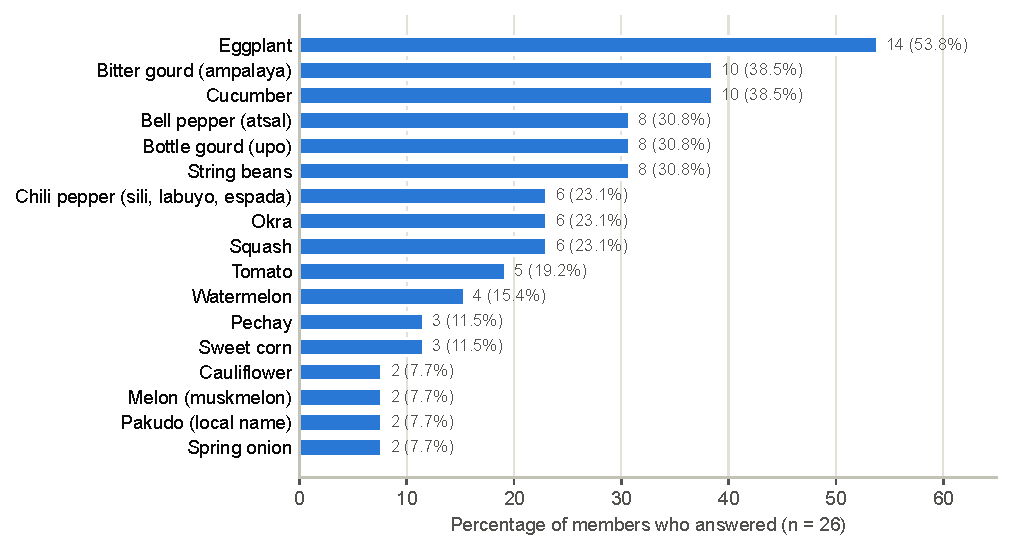
\includegraphics[width=0.86\linewidth]{figures/fig_crops.pdf}
\caption{Crops produced by the members (multiple response; \textit{n} = 26 who answered). Crops named by only one member are not shown: cabbage, calamansi, lettuce, Malabar spinach (\textit{alugbati}), mixed \textit{pinakbet} vegetables, sponge gourd (\textit{sikwa}), and sweet potato. ``Pakudo'' is a local crop name that could not be identified.}
\label{fig:crops}
\end{figure}

Pests are the most common problem in planting (Table~\ref{tab:problems}). Every member who answered had problems with insects or pests, and almost three in four also had plant disease. A few members wrote in other problems: typhoons, white flies, and theft by neighbors.

\begin{table}[H]
\centering
\begin{threeparttable}
\caption{Problems encountered in planting (multiple response; \textit{n} = 26 who answered)}
\label{tab:problems}
\small
\begin{tabular}{p{5.2cm}rr}
\toprule
Problem & \textit{f} & \%\\
\midrule
Insects and pests & 26 & 100.00\\
Plant disease & 19 & 73.08\\
Others & 9 & 34.62\\
\quad Typhoon & 1 & 3.85\\
\quad White flies & 1 & 3.85\\
\quad Theft by neighbors & 1 & 3.85\\
\quad Not specified & 6 & 23.08\\
\bottomrule
\end{tabular}
\end{threeparttable}
\end{table}

\subsection{Perceived usability of the platform (SUS)}

The members gave a mean SUS score of \textbf{54.40} (Table~\ref{tab:sus}). This score is rated \textbf{``OK''}, falls in the \textbf{low marginal} range of acceptability, and earns a \textbf{grade of D}, which is below the benchmark average of 68. The scores were close together (\textit{SD} = 7.93): 21 of the 26 members scored in the ``OK'' band, and only one member scored in the acceptable range (Figure~\ref{fig:susdist}). Appendix~A lists each member's score.

\begin{table}[H]
\centering
\begin{threeparttable}
\caption{SUS scores of the members and the administrator}
\label{tab:sus}
\small
\begin{tabularx}{0.9\linewidth}{lLL}
\toprule
 & Members (\textit{n} = 26) & Administrator (\textit{n} = 1)\\
\midrule
Mean SUS score & \textbf{54.40} (\textit{SD} = 7.93) & \textbf{82.50}\\
Median; range & 52.50; 35.00--77.50 & --\\
95\% confidence interval & 51.20--57.61 & --\\
Adjective rating \citep{bangor2009} & OK & Excellent\\
Acceptability \citep{bangor2008} & Marginal (low) & Acceptable\\
Grade \citep{sauro2016} & D (15th--34th percentile) & A (90th--95th percentile)\\
\bottomrule
\end{tabularx}
\end{threeparttable}
\end{table}

\begin{figure}[H]
\centering
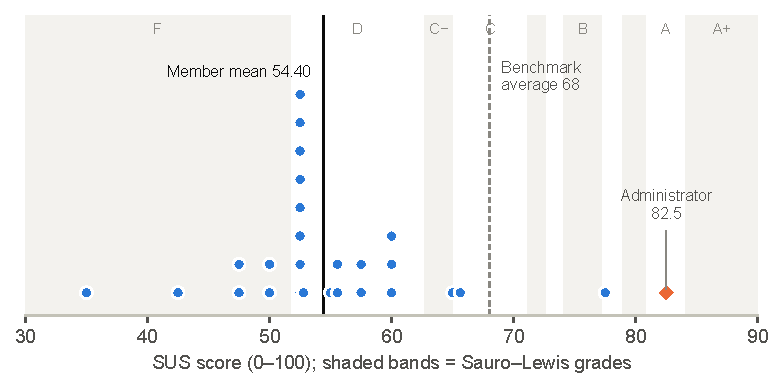
\includegraphics[width=0.9\linewidth]{figures/fig_sus_distribution.pdf}
\caption{SUS scores of the 26 members (blue dots; scores that are the same are stacked) and of the administrator (orange diamond). The shaded bands mark the letter grades of the curved grading scale.}
\label{fig:susdist}
\end{figure}

\textbf{What lowered the score?} Figure~\ref{fig:susitems} shows the members' answers to each SUS item. Most members agreed with the positive statements. For example, 84\% felt confident using the app and 76\% would like to use it frequently. However, many members also agreed with the negative statements: 69\% said they would need the support of a technical person, and 65\% said they needed to learn a lot before they could use the app. These two items lowered the SUS score the most.

\begin{figure}[H]
\centering
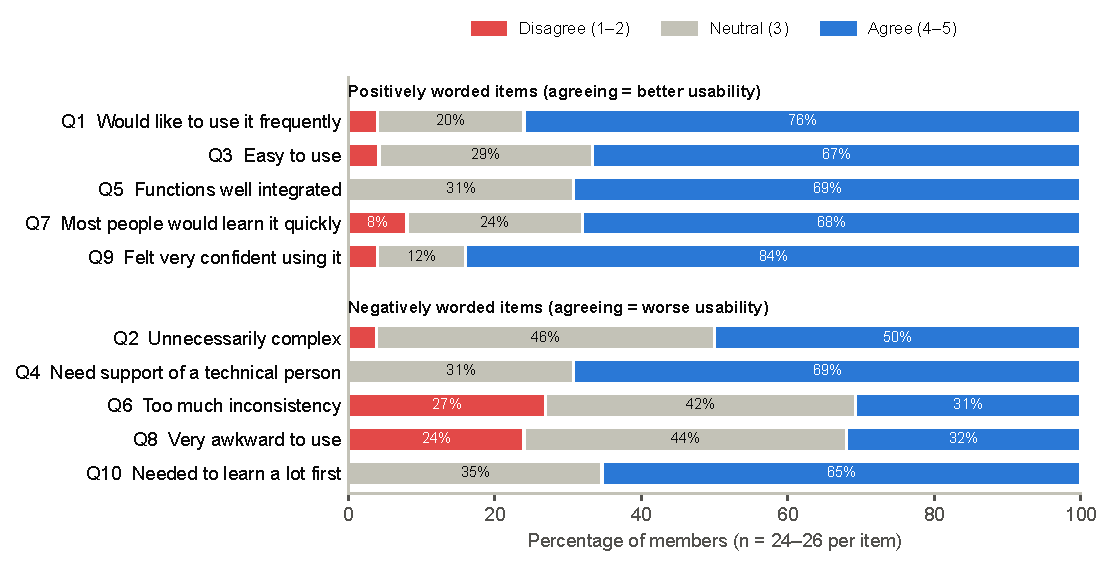
\includegraphics[width=0.94\linewidth]{figures/fig_sus_items.pdf}
\caption{Members' answers to the ten SUS items. For the negatively worded items, agreeing means a \textit{worse} experience.}
\label{fig:susitems}
\end{figure}

\textbf{How to read the SUS result.} Two things should be kept in mind.
\begin{itemize}
  \item \textit{Some members may have misread the negative statements.} Of the 16 members who agreed that the app was easy to use, 13 also agreed that it was unnecessarily complex or very awkward to use. Because of this, the ten items did not hang together well in this group (Cronbach's $\alpha$ = .42, compared with about .90 in typical SUS studies; \citealt{bangor2008}). Respondents are known to make this kind of mistake on questionnaires that switch between positive and negative wording \citep{sauro2011}, and it may be more likely here because the farmers answered a translated form. If so, the true usability is probably somewhat higher than 54.40, and the score is best read as a conservative estimate.
  \item \textit{The need for help is still real.} The SUS score correlated with the members' ease-of-use ratings (Spearman's $\rho$ = .45, \textit{p} = .024, \textit{n} = 25), so it still ranks the members sensibly. One member also commented that the app suits ``those who are used to phones.'' The members' agreement that they need support and training should therefore be acted on.
\end{itemize}

\subsection{Perceived usefulness, ease of use, and intention to use}

The members gave clearly positive answers on the 1--7 items (Table~\ref{tab:tam} and Figure~\ref{fig:tam}). Overall, they \textbf{agreed} with the statements (mean 5.42).

\begin{table}[H]
\centering
\begin{threeparttable}
\caption{Members' ratings of usefulness, ease of use, and intention to use}
\label{tab:tam}
\small
\begin{tabularx}{\linewidth}{lLcccl}
\toprule
 & Statement & \textit{n} & Mean & \textit{SD} & Interpretation\\
\midrule
\multicolumn{6}{l}{\textit{Perceived usefulness} (\textit{n} = 26; $\alpha$ = .86)}\\
Q1 & Using the application allows me to place orders more quickly. & 25 & 5.32 & 1.41 & Agree\\
Q2 & Using the application makes it more convenient for me to order products from \textit{Baybayani}. & 25 & 5.56 & 1.08 & Agree\\
Q3 & Using the application helps me keep track of my orders. & 25 & 5.60 & 1.00 & Agree\\
Q4 & Using the application improves my overall online shopping experience. & 26 & 5.50 & 1.27 & Agree\\
Q5 & I find the application useful for buying products from \textit{Baybayani}. & 27 & 5.70 & 1.30 & Agree\\
 & \textbf{Construct mean} & & \textbf{5.55} & \textbf{0.97} & \textbf{Agree}\\
\addlinespace
\multicolumn{6}{l}{\textit{Perceived ease of use} (\textit{n} = 27; $\alpha$ = .84)}\\
Q6 & Learning to use the application was easy for me. & 26 & 5.42 & 1.55 & Agree\\
Q7 & I find it easy to find the products I want. & 27 & 5.63 & 1.18 & Agree\\
Q8 & I find the ordering and checkout process easy to follow. & 27 & 5.22 & 1.19 & Slightly agree\\
Q9 & The user interface of the application is easy to understand. & 25 & 5.00 & 1.38 & Slightly agree\\
Q10 & It is easy for me to become skillful at using the application. & 27 & 5.00 & 1.30 & Slightly agree\\
 & \textbf{Construct mean} & & \textbf{5.25} & \textbf{1.00} & \textbf{Slightly agree}\\
\addlinespace
\multicolumn{6}{l}{\textit{Intention to use or recommend} (\textit{n} = 25; $\alpha$ = .69)}\\
Q11 & I intend to use the application for my future orders. & 25 & 5.32 & 1.52 & Agree\\
Q12 & I prefer ordering through the application over buying in person. & 24 & 5.21 & 1.10 & Slightly agree\\
Q13 & I would recommend the application to other people. & 25 & 5.68 & 1.25 & Agree\\
 & \textbf{Construct mean} & & \textbf{5.42} & \textbf{1.02} & \textbf{Agree}\\
\addlinespace
 & \textbf{All 13 items} (\textit{n} = 26; $\alpha$ = .94) & & \textbf{5.42} & \textbf{0.90} & \textbf{Agree}\\
\bottomrule
\end{tabularx}
\begin{tablenotes}\footnotesize
\item \textit{Note.} Item \textit{n} varies because some items were left blank. Construct means are the averages of the respondents' construct scores. Each $\alpha$ is based on the members who answered every item of the construct.
\end{tablenotes}
\end{threeparttable}
\end{table}

\begin{figure}[H]
\centering
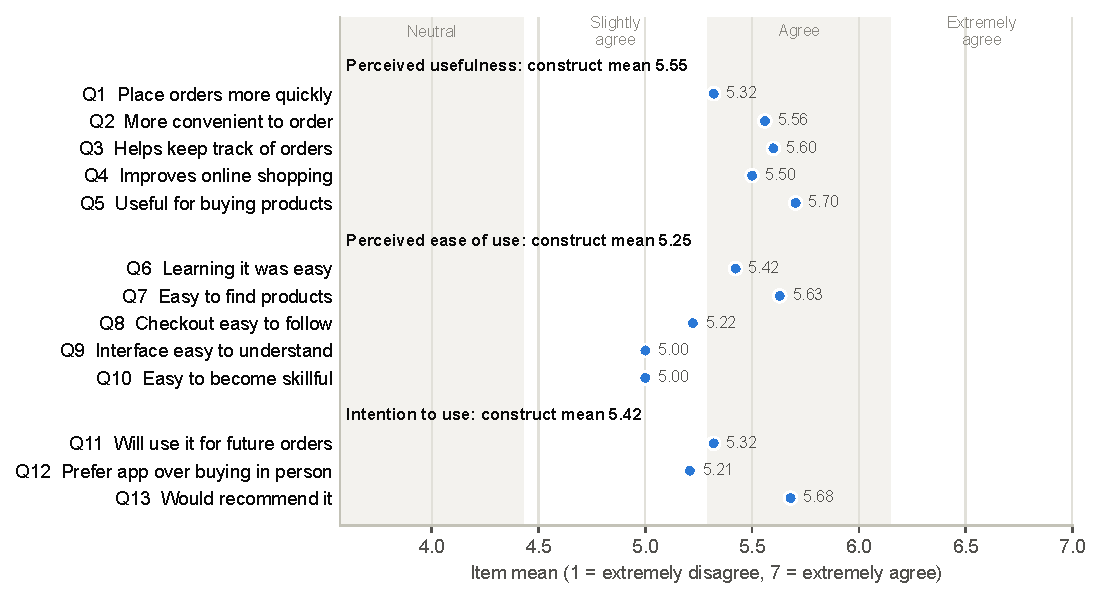
\includegraphics[width=0.9\linewidth]{figures/fig_part2b_items.pdf}
\caption{Members' mean rating of each item. The shaded and unshaded bands show the interpretation scale in Table~\ref{tab:scale}.}
\label{fig:tam}
\end{figure}

\textbf{Usefulness was rated highest} (5.55, agree). The members found the app useful for buying from \textit{Baybayani} (5.70), helpful for keeping track of their orders (5.60), and a more convenient way to order from \textit{Baybayani} (5.56).

\textbf{Intention to use was also positive} (5.42, agree). The members were most willing to recommend the app to others (5.68). They were less sure that they would choose the app over buying in person (5.21, slightly agree).

\textbf{Ease of use was rated lowest} (5.25, slightly agree). Finding products was rated easy (5.63). However, understanding the interface (5.00), becoming skillful with the app (5.00), and following the checkout process (5.22) received only slight agreement. This matches the SUS finding that members want more guidance.

The items were reliable. Alpha was good for usefulness (.86) and ease of use (.84) and excellent for all 13 items together (.94). It was slightly below the acceptable level for the three-item intention scale (.69), which is common for very short scales. Across the constructs, about half to two-thirds of the members were in the ``agree'' or ``extremely agree'' range, and only one or two members per construct scored below neutral.

\subsection{Administrator's evaluation}

Because there is only one administrator, the results in Table~\ref{tab:admin} describe one person's view and are not an average. The administrator gave a SUS score of \textbf{82.50}, rated \textbf{Excellent}, with a \textbf{grade of A}. Unlike many members, the administrator answered the positive and negative statements consistently. For example, the administrator disagreed that they needed technical support or needed to learn a lot first.

\begin{table}[H]
\centering
\begin{threeparttable}
\caption{Administrator's ratings of usefulness, ease of use, and intention to use (\textit{n} = 1)}
\label{tab:admin}
\small
\begin{tabularx}{\linewidth}{lLcl}
\toprule
 & Statement & Rating & Interpretation\\
\midrule
\multicolumn{4}{l}{\textit{Perceived usefulness} (mean 7.00, extremely agree)}\\
Q1 & Using the application helps me record orders more accurately. & 7 & Extremely agree\\
Q2 & Using the application allows me to manage orders more quickly. & 7 & Extremely agree\\
Q3 & Using the application makes retrieving order records easier. & 7 & Extremely agree\\
Q4 & Using the application helps me generate order reports and summaries. & 7 & Extremely agree\\
Q5 & I find the application useful for performing my tasks. & 7 & Extremely agree\\
\addlinespace
\multicolumn{4}{l}{\textit{Perceived ease of use} (mean 5.60, agree)}\\
Q6 & Learning to use the administrator features was easy for me. & 6 & Agree\\
Q7 & I find it easy to view and update order information. & 7 & Extremely agree\\
Q8 & The administrator interface is clear and understandable. & 7 & Extremely agree\\
Q9 & Interacting with the application requires little mental effort. & 2 & Disagree\\
Q10 & It is easy for me to get the application to do what I need it to do. & 6 & Agree\\
\addlinespace
\multicolumn{4}{l}{\textit{Intention to use or recommend} (mean 6.67, extremely agree)}\\
Q11 & I intend to continue using the application for tracking the organization's orders. & 7 & Extremely agree\\
Q12 & I prefer using the application over my current method of recording orders. & 6 & Agree\\
Q13 & I would recommend the continued use of the application in the organization. & 7 & Extremely agree\\
\addlinespace
 & \textbf{All 13 items} & \textbf{6.38} & \textbf{Extremely agree}\\
\bottomrule
\end{tabularx}
\end{threeparttable}
\end{table}

The administrator gave the top rating (7) to every usefulness item: recording, managing, retrieving, and reporting orders. They intend to keep using the system and would recommend it to the organization. The one weak point is effort. The administrator found the interface clear (7), but disagreed that using the system takes little mental effort (2) and agreed that it is unnecessarily complex (SUS item 2). The back-office tasks work well, but they could be made lighter.

\subsection{Comments and suggestions}

Eight of the 28 respondents wrote a comment. One member wrote ``no comment,'' and the rest left the item blank. Table~\ref{tab:comments} groups the comments by theme.

\begin{table}[H]
\centering
\begin{threeparttable}
\caption{Themes in the respondents' comments}
\label{tab:comments}
\small
\begin{tabularx}{\linewidth}{>{\raggedright\arraybackslash}p{3.4cm}>{\raggedright\arraybackslash}p{2.4cm}L}
\toprule
Theme & Respondents & What was said\\
\midrule
Satisfaction and endorsement & R04, R21, R22, R23, R26 & Satisfied with the app; good for buying vegetables more easily; convenient for those used to phones; would strongly recommend it to friends.\\
Payment options & R01 (administrator) & Add online payment through GCash, Maya, and MariBank.\\
Order handling & R20 & Show the customer's address and a pick-up time so the store can prepare and prioritize orders.\\
Continued improvement & R26 & The app is good but still needs to be improved.\\
Beyond the app & R11 & Promote value-adding of vegetable products.\\
\bottomrule
\end{tabularx}
\begin{tablenotes}\footnotesize
\item \textit{Note.} The comments of R22 and R23 are almost word for word the same. Cebuano comments were translated into English.
\end{tablenotes}
\end{threeparttable}
\end{table}

The comments were few but mostly positive, which agrees with the ratings. The specific suggestions are about payment and order logistics, and they can be turned directly into features for the next version.

% =====================================================================
\section{Conclusions and Recommendations}

\subsection{Conclusions}
\begin{enumerate}
  \item The members find the \textit{Baybayani} platform \textbf{useful} and \textbf{intend to keep using and recommending it}. Their overall rating was 5.42 out of 7 (agree).
  \item The members' perceived usability is \textbf{marginal} (SUS 54.40, ``OK,'' grade D). Part of this low score likely comes from misreading the negatively worded items, but the members also clearly feel that they need \textbf{support and training} to use the app well.
  \item \textbf{Ease of use} is the weakest area for members, especially understanding the interface, becoming skillful with the app, and following the checkout process.
  \item The administrator rates the system as \textbf{excellent} (SUS 82.50, grade A) and \textbf{extremely useful} for managing orders, but finds that the work takes considerable mental effort.
\end{enumerate}

\subsection{Recommendations}
\begin{enumerate}
  \item \textbf{Train and support the members.} Hold hands-on orientation sessions, prepare a short illustrated guide in Cebuano, and assign a contact person, such as an officer, whom members can ask for help.
  \item \textbf{Simplify ordering and checkout,} and review the wording of the interface in Cebuano.
  \item \textbf{Add the requested features:} e-wallet payment (GCash, Maya, MariBank), the customer's delivery address, and pick-up scheduling for order preparation.
  \item \textbf{Make the administrator's work lighter} by streamlining the most frequent order tasks.
  \item \textbf{In future evaluations,} use the all-positive version of the SUS \citep{sauro2011} or read the items aloud in Cebuano, to reduce errors on the negatively worded items.
\end{enumerate}

\subsection{Limitations}
The members were a small convenience sample (\textit{n} = 27), and there was only one administrator, so the results describe this group and should not be generalized to all users. The SUS showed low internal consistency in this sample, so the member SUS score should be read together with the 1--7 ratings. Income and years of membership are the respondents' own estimates, and a third of the members did not report their income. Finally, two members gave the same answer to all 13 items, and two members wrote nearly identical comments, which suggests that a few respondents answered quickly or together.

% =====================================================================
\begin{thebibliography}{9}
\setlength{\itemsep}{2pt}
\small

\bibitem[Bangor et~al.(2008)]{bangor2008}
Bangor, A., Kortum, P.~T., \& Miller, J.~T. (2008). An empirical evaluation of the System Usability Scale. \textit{International Journal of Human--Computer Interaction, 24}(6), 574--594.

\bibitem[Bangor et~al.(2009)]{bangor2009}
Bangor, A., Kortum, P., \& Miller, J. (2009). Determining what individual SUS scores mean: Adding an adjective rating scale. \textit{Journal of Usability Studies, 4}(3), 114--123.

\bibitem[Brooke(1996)]{brooke1996}
Brooke, J. (1996). SUS: A ``quick and dirty'' usability scale. In P.~W. Jordan, B. Thomas, B.~A. Weerdmeester, \& I.~L. McClelland (Eds.), \textit{Usability evaluation in industry} (pp.~189--194). Taylor \& Francis.

\bibitem[Davis(1989)]{davis1989}
Davis, F.~D. (1989). Perceived usefulness, perceived ease of use, and user acceptance of information technology. \textit{MIS Quarterly, 13}(3), 319--340.

\bibitem[George \& Mallery(2003)]{george2003}
George, D., \& Mallery, P. (2003). \textit{SPSS for Windows step by step: A simple guide and reference, 11.0 update} (4th ed.). Allyn \& Bacon.

\bibitem[Sauro \& Lewis(2011)]{sauro2011}
Sauro, J., \& Lewis, J.~R. (2011). When designing usability questionnaires, does it hurt to be positive? In \textit{Proceedings of the SIGCHI Conference on Human Factors in Computing Systems} (pp.~2215--2224). ACM.

\bibitem[Sauro \& Lewis(2016)]{sauro2016}
Sauro, J., \& Lewis, J.~R. (2016). \textit{Quantifying the user experience: Practical statistics for user research} (2nd ed.). Morgan Kaufmann.

\end{thebibliography}

% =====================================================================
\appendix
\section*{Appendix A. SUS score of each member}
\addcontentsline{toc}{section}{Appendix A. SUS score of each member}

\begin{table}[H]
\centering
\begin{threeparttable}
\small
\setlength{\tabcolsep}{5pt}
\begin{tabular}{lcrll@{\hspace{2.2em}}lcrll}
\toprule
Code & Items & SUS & Rating & Grade & Code & Items & SUS & Rating & Grade\\
\midrule
R02 & 10 & 65.00 & Good & C & R16 & 10 & 52.50 & OK & D\\
R03 & 10 & 57.50 & OK & D & R17 & 10 & 52.50 & OK & D\\
R04 & 10 & 55.00 & OK & D & R18 & 10 & 35.00 & Poor & F\\
R05 & 10 & 77.50 & Good & B+ & R19 & 9 & 55.56\tnote{a} & OK & D\\
R06 & 10 & 47.50 & OK & F & R20 & 10 & 52.50 & OK & D\\
R07 & 8 & 65.63\tnote{a} & Good & C & R21 & 9 & 50.00\tnote{a} & OK & F\\
R08 & 10 & 47.50 & OK & F & R22 & 10 & 60.00 & OK & D\\
R09 & 10 & 52.50 & OK & D & R23 & 10 & 52.50 & OK & D\\
R10 & 10 & 57.50 & OK & D & R24 & 9 & 55.56\tnote{a} & OK & D\\
R11 & 10 & 50.00 & OK & F & R25 & 9 & 52.78\tnote{a} & OK & D\\
R12 & 10 & 42.50 & Poor & F & R26 & 10 & 60.00 & OK & D\\
R13 & 10 & 60.00 & OK & D & R27 & 10 & 52.50 & OK & D\\
R14 & 0 & -- & -- & -- & R28 & 10 & 52.50 & OK & D\\
R15 & 10 & 52.50 & OK & D & & & & & \\
\bottomrule
\end{tabular}
\begin{tablenotes}\footnotesize
\item \textit{Note.} Items = number of SUS items answered. Rating = adjective rating \citep{bangor2009}; Grade = curved grade \citep{sauro2016}. R14 left the SUS page blank.
\item[a] Prorated from the items answered.
\end{tablenotes}
\end{threeparttable}
\end{table}

\end{document}
